 \section{Creare applicazioni C++}

Non tutti vogliono un'applicazione GIS completa. Talvolta si vuole solamente avere un widget nella propria applicazione che mostri una mappa mentre lo scopo principale dell'applicazione è un altro. Forse un database frontend con un mappa? Questa Sezione fornisce due semplici esempi di scritti da Tim Sutton.
Sono disponibili nell'archivio QGIS subversion insieme con altre interessanti guide. L'intero archivio può essere esplorato: 
\filename{https://svn.osgeo.org/qgis/trunk/code\_examples/}

\subsection{Creare un semplice widget mappa}\label{subsec:simple_widget}

Con questa guida si esplora come creare un semplice widget di mappazione. Non farà molto, solo caricare uno shape file e mostrarlo in colori casuali. Ma dovrebbe dare un'idea delle potenzialità di QGIS con un componente di mappazione incorporato. Prima di procedere, molti ringraziamenti a Francis Bolduc che ha scritto l'inizio di questa demo. Egli ha gentilmente acconsentito a rendere il suo lavoro pubblicamente disponibile.

Si comincia con la tipica aggiunta dei necessari "includes" per la nostra applicazione:

\begin{verbatim}
//
// QGIS Includes
//
#include <qgsapplication.h>
#include <qgsproviderregistry.h>
#include <qgssinglesymbolrenderer.h>
#include <qgsmaplayerregistry.h>
#include <qgsvectorlayer.h>
#include <qgsmapcanvas.h>
//
// Qt Includes
//
#include <QString>
#include <QApplication>
#include <QWidget>
\end{verbatim}

Si usa QgsApplication invece di Qt's QApplication, e si ottengono alcuni benefici aggiuntivi di vari metodi statici che possono essere usati per localizzare i percorsi della libreria e così via.

Il registro del provider è un singleton che tiene traccia dei plugin del provider di dati vettoriali. Fa tutto il lavoro di caricare i plugin e così via. Il generatore di singolo simbolo è la più basilare classe di simbologia. Genera punti linee o poligoni in un singolo colore che viene scelto a priori in modo casuale (anche se lo si può impostare in modo personalizzato). Ogni layer vettoriale deve avere una simbologia da esso associata.

Il registro del layer di mappa tiene traccia di tutti i layer in uso. La classe del layer vettoriale eredita da maplayer e lo estende ad includere funzionalità specialistiche per dati vettoriali.

Infine il mapcanvas è realmente il nocciolo della questione. È un widget disegnabile su cui sarà disegnata la mappa.

Ora si può andare oltre alla inizializzazione della nostra applicazione....

\begin{verbatim}
int main(int argc, char ** argv)
{
  // Start the Application
  QgsApplication app(argc, argv, true);

  QString myPluginsDir        = "/home/timlinux/apps/lib/qgis";
  QString myLayerPath         = "/home/timlinux/gisdata/brazil/BR_Cidades/";
  QString myLayerBaseName     = "Brasil_Cap";
  QString myProviderName      = "ogr";

\end{verbatim}

Così ora abbiamo un'applicazione qgs e abbiamo definito alcune variabili. Dato che ho testato su Ubuntu 8.10, specifico qui le posizione dei plugin del provider vettoriale come nella mia directory di installazione sviluppo. Probabilmente avrebbe più senso in generale tenere le librerie QGIS libs in uno dei percorsi di ricerca delle library standard del vostro sistema (ad es. /usr/lib) ma per ora andrà bene anche così.

Le prossime due variabili definite qui indicano solo il file shape che si userà (e qui dovreste sostituire i vostri dati).

Il nome del provider è importante: dice a QGIS che provider di dati usare per caricare il file. Tipicamente si userà 'ogr' o 'postgres'.

Ora possiamo creare il layer oggetto.

\begin{verbatim}
  // Instantiate Provider Registry
  QgsProviderRegistry::instance(myPluginsDir);
\end{verbatim}

Prima si inizializza il registro del provider. È una classe singleton quindi si usa un'istanza di chiamata statica e si passa il percorso di ricerca della library del provider. Appena inizializzato scansionerà questo percorso alla ricerca di lbrerie del provider.

Ora si crea un layer...

\begin{verbatim}
  QgsVectorLayer * mypLayer =
      new QgsVectorLayer(myLayerPath, myLayerBaseName, myProviderName);
  QgsSingleSymbolRenderer *mypRenderer = new
QgsSingleSymbolRenderer(mypLayer->geometryType());
  QList <QgsMapCanvasLayer> myLayerSet;

  mypLayer->setRenderer(mypRenderer);
  if (mypLayer->isValid())
  {
    qDebug("Layer is valid");
  }
  else
  {
    qDebug("Layer is NOT valid");
  }

  // Add the Vector Layer to the Layer Registry
  QgsMapLayerRegistry::instance()->addMapLayer(mypLayer, TRUE);
  // Add the Layer to the Layer Set
  myLayerSet.append(QgsMapCanvasLayer(mypLayer, TRUE));

\end{verbatim}

Il codice è adeguatamente auto esplicativo qui. Si crea un layer usando le variabili definite prima. Poi si assegna al layer un generatore di immagini. Quando si crea un generatore di immagini, dobbiamo specificare il tipo di geometria, cosa che si fa chiedendo allo stato vettoriale il suo tipo di geometria. Poi si aggiunge il layer ad un set di layer (che è usato da QgsMapCanvas per tenere traccia di quali layer generare graficamente e in che ordine) e al registro di maplayer. Infine ci si assicura che il layer sarà visibile.
Ora si crea un map canvas sul quale disegnare il layer.

\begin{verbatim}
  // Create the Map Canvas
  QgsMapCanvas * mypMapCanvas = new QgsMapCanvas(0, 0);
  mypMapCanvas->setExtent(mypLayer->extent());
  mypMapCanvas->enableAntiAliasing(true);
  mypMapCanvas->setCanvasColor(QColor(255, 255, 255));
  mypMapCanvas->freeze(false);
  // Set the Map Canvas Layer Set
  mypMapCanvas->setLayerSet(myLayerSet);
  mypMapCanvas->setVisible(true);
  mypMapCanvas->refresh();

\end{verbatim}

Di nuovo, non c'è niente di particolarmente complesso in questo. Si crea il canvas e si imposta la sua estensione a quella del layer. Poi si aggiusta un po' il canvas per disegnare vettori a distorsione minima. Infine si imposta il colore di sfondo, si sblocca il canvas, si rende visibile e quindi si aggiorna.

\begin{verbatim}
  // Start the Application Event Loop
  return app.exec();
}

\end{verbatim}

Nell'ultimo passaggio semplicemente si avvia il loop di eventi Qt ed è fatta. Si può controllare, compilare e lanciare usando cmake come questo:

\begin{verbatim}
svn co
https://svn.osgeo.org/qgis/trunk/code_examples/1_hello_world_qgis_style
cd 1_hello_world_qgis_style
mkdir build
#optionally specify where your QGIS is installed (should work on all
platforms)
#if your QGIS is installed to /usr or /usr/local you can leave this next step
out
export LIB_DIR=/home/timlinux/apps
cmake ..
make
./timtut1
\end{verbatim}

Quando lo si compila e lo si lancia ecco come appare l'applicazione funzionante:

\begin{figure}[ht]
   \begin{center}
   \caption{Semplice applicazione C++ \osxcaption}\label{fig:cpp1_application}\smallskip
   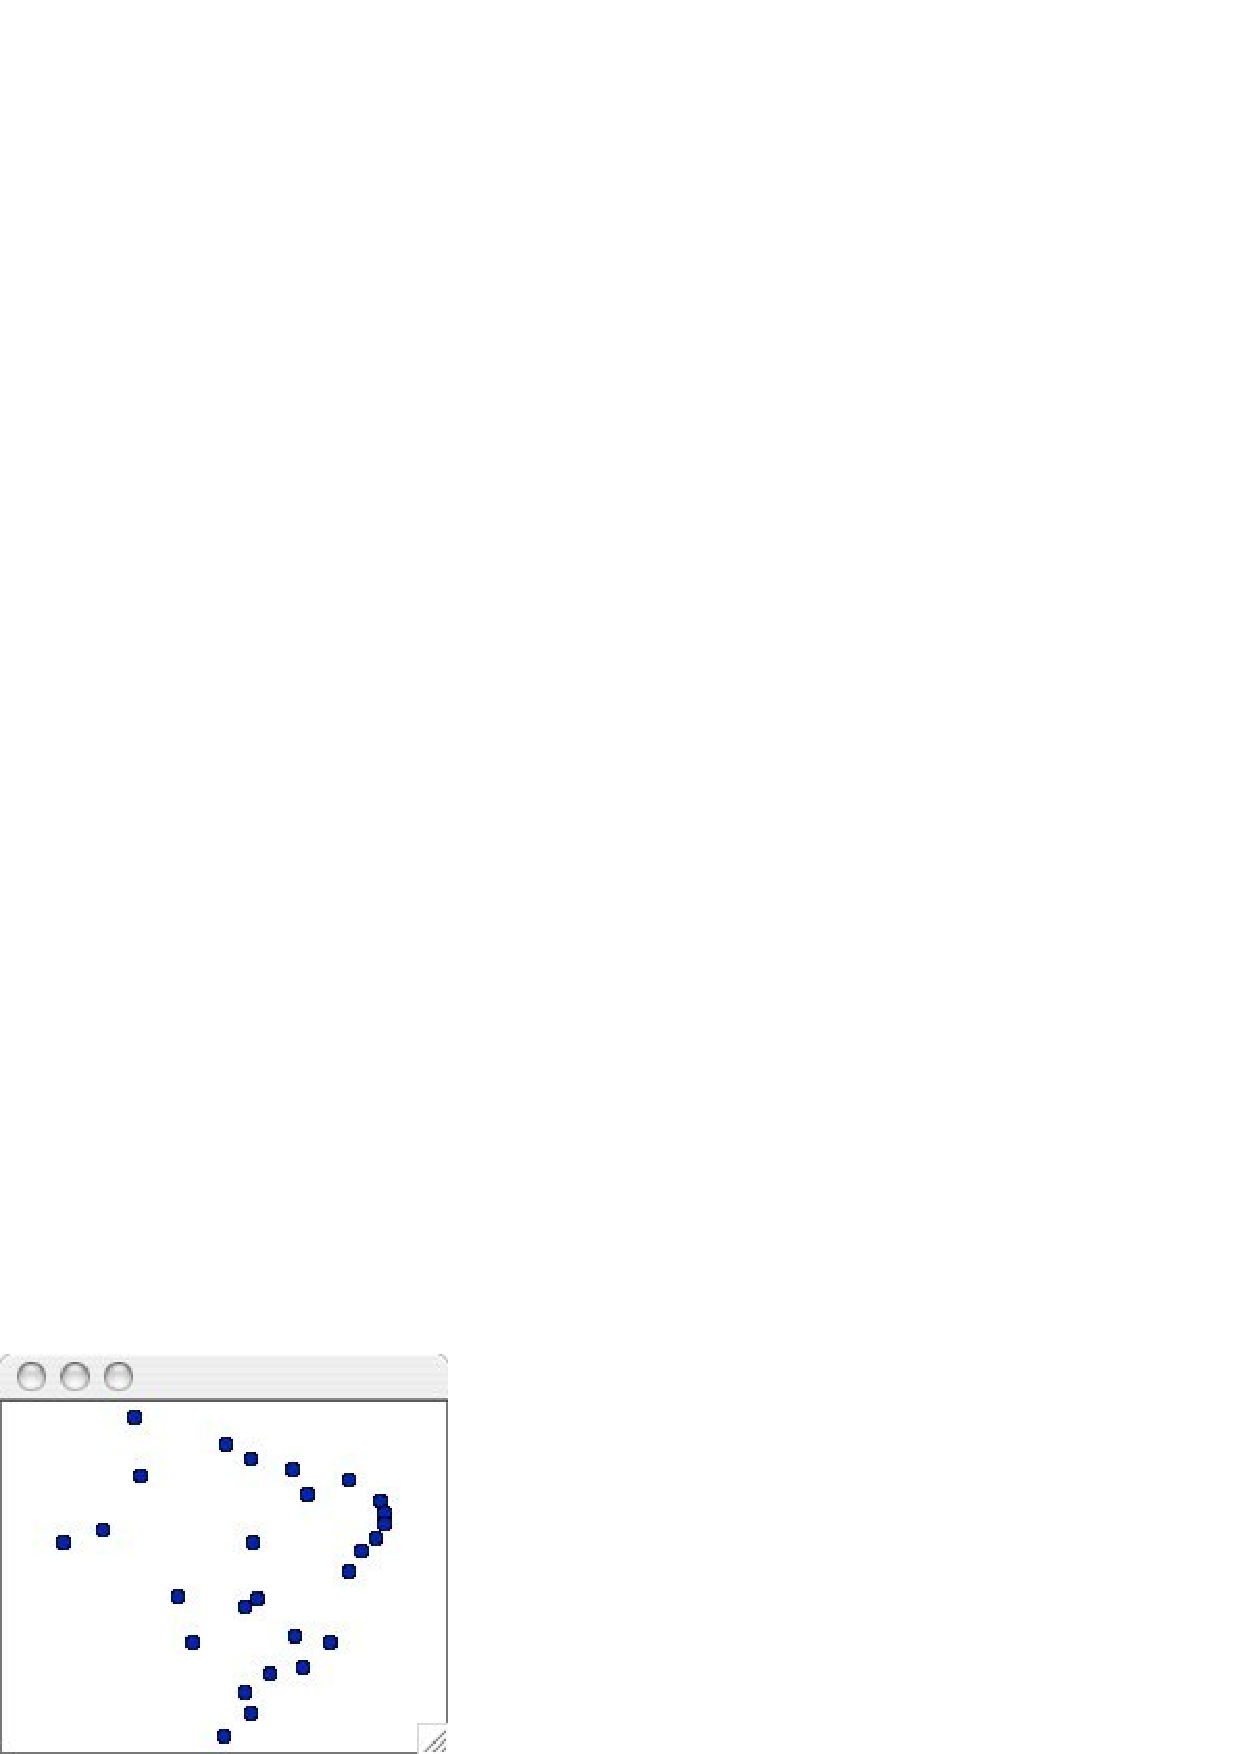
\includegraphics[clip=true]{cpp1_application}
\end{center}
\end{figure}

\subsection{Lavorare con QgsMapCanvas}

nella Sezione~\ref{subsec:simple_widget} è stato illustrato l'uso del QgsMapCanvas api per creare una semplice applicazione che carica un file shape e mostra i punti in esso contenuti. Ma a cosa serve una mappa con la quale non si può interagire?

In questa seconda guida la guida precedente viene estesa rendendola un'applicazione QMainWindow con un menu, una barra degli strumenti e un'area canvas. Si illustra come usare QgsMapTool - la classe base per tutti gli strumenti che devono interagire con il canvas della mappa.
Lo scopo è fornire un progetto dimostrativo, così non prometto di scrivere il più elegante o il più robusto dei codici C++. Il progetto fornirà 4 icon per barre degli strumenti per

\begin{itemize}
 \item caricare un layer mappa (il nome del layer è incorporato nell'applicazione)
 \item ingrandire
 \item ridurre
 \item panoramica
\end{itemize}

Nella directory di lavoro per il codice guida si trovano un certo numero di file incluse sorgenti c++, icone e un semplice file di dati sotto il nome dati. C'è anche il file .ui per la finestra principale.

\textbf{Nota:} Sarà necessario editare il file .pro nella directory svn soprastante per abbinarlo al proprio sistema.

dato che il codice è lo stesso della precedente guida, ci focalizzeremo sulle specifiche MapTool - il resto dei dettagli di implementazione può essere investigato esplorando il progetto da SVN. Un QgsMapTool è una clasee che interagisce con il MapCanvas usando il puntatore del mouse. QGIS ha un gran numero di QgsMapTools implementati, e si possono fare delle sottoclassi in QgsMapTool per crearsi i propri. In mainwindow.cpp si può vedere che ho incluso dei capipagina per il QgsMapTools vicino all'inzio del file:

\begin{verbatim}
     //
     // QGIS Map tools
     //
     #include "qgsmaptoolpan.h"
     #include "qgsmaptoolzoom.h"
     //
     // These are the other headers for available map tools 
     // (not used in this example)
     //
     //#include "qgsmaptoolcapture.h"
     //#include "qgsmaptoolidentify.h"
     //#include "qgsmaptoolselect.h"
     //#include "qgsmaptoolvertexedit.h"
     //#include "qgsmeasure.h"
\end{verbatim}

Come si vede, uso soltanto due tipi di sottoclassi MapTool per questa guida, ma ce ne sono altre disponibili nella libreria QGIS. Collegare MapTools al canvas è molto semplice usando il normale meccanismo Qt4 segnale/slot:

\begin{verbatim}
     //create the action behaviours
     connect(mActionPan, SIGNAL(triggered()), this, SLOT(panMode()));
     connect(mActionZoomIn, SIGNAL(triggered()), this, SLOT(zoomInMode()));
     connect(mActionZoomOut, SIGNAL(triggered()), this, SLOT(zoomOutMode()));
     connect(mActionAddLayer, SIGNAL(triggered()), this, SLOT(addLayer()));
\end{verbatim}

Quindi si crea una piccola barra degli strumenti per contenere i pulsanti degli strumenti. Da notare che le azioni mpAction* sono state create in designer.

\begin{verbatim}
     //create a little toolbar
     mpMapToolBar = addToolBar(tr("File"));
     mpMapToolBar->addAction(mpActionAddLayer);
     mpMapToolBar->addAction(mpActionZoomIn);
     mpMapToolBar->addAction(mpActionZoomOut);
     mpMapToolBar->addAction(mpActionPan);
\end{verbatim}

Anche la parte Qt è decisamente diretta. Ora si creano tre strumenti della mappa:

\begin{verbatim}
     //create the maptools
     mpPanTool = new QgsMapToolPan(mpMapCanvas);
     mpPanTool->setAction(mpActionPan);
     mpZoomInTool = new QgsMapToolZoom(mpMapCanvas, FALSE); // false = in
     mpZoomInTool->setAction(mpActionZoomIn);
     mpZoomOutTool = new QgsMapToolZoom(mpMapCanvas, TRUE ); //true = out
     mpZoomOutTool->setAction(mpActionZoomOut);
\end{verbatim}

Di nuovo, niente qui è molto complicato - si creano le istanze degli strumenti, ognuno dei quali è associato con lo stesso mapcanvas, ed una diversa QAction. Quando l'utente seleziona una delle icone della barra degli strumenti, il MapTool attivo per il canvas viene impostato. Per esempio, quando l'icona panoramica viene premuta, si fa questo:

\begin{verbatim}
    void MainWindow::panMode()
    {
       mpMapCanvas->setMapTool(mpPanTool); 
    }
\end{verbatim}

\begin{figure}[ht]
   \begin{center}
   \caption{Applicazione QMainWindow con un menu, una barra degli strumenti e un'area canvas
\osxcaption}\label{fig:cpp2_application}\smallskip
   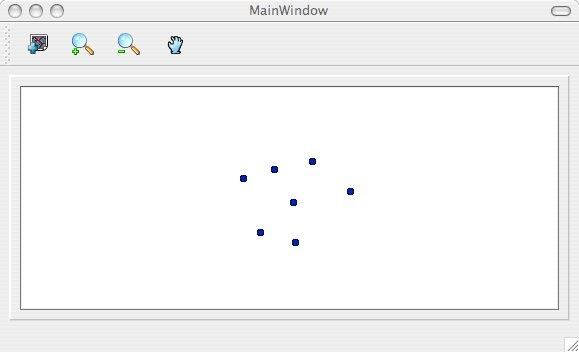
\includegraphics[clip=true, width=\textwidth]{cpp2_application}
\end{center}
\end{figure}

\minisec{Conclusioni}

Come si vede, ampliare il precedente esempio a qualcosa di più funzionale usando MapTools è veramente molto facile e richiede solo poche righe di codice per ogni MapTool che si voglia fornire.

Si può controllare e costruire questa guida usando SVN e CMake usando i seguenti passaggi:

\begin{verbatim}
svn co https://svn.osgeo.org/qgis/trunk/code_examples/2_basic_main_window
cd 2_basic_main_window
mkdir build
#optionally specify where your QGIS is installed (should work on all platforms)
#if your QGIS is installed to /usr or /usr/local you can leave this next step out
export LIB_DIR=/home/timlinux/apps
cmake ..
make
./timtut2
\end{verbatim}


